% Introductory slides; included by main.tex.
\begin{frame}[plain]
        \begin{tikzpicture}[remember picture,overlay]
                \node[anchor=north east,inner sep=0pt] at
                ([xshift=-5mm,yshift=-4mm]current page.north east)
                {\alicelogo{15mm}\hspace{5mm}
\includegraphics[height=12mm]{slides/assets/tum-logo.pdf}};
        \end{tikzpicture}
        \titlepage
        \centering\small A demonstration of the workflow: local
        processing and Hyperloop.
\end{frame}

\begin{frame}{Why a dedicated data format for femto analysis?}
        \begin{block}{Large datasets, many analyses}
                Large datasets reach the petabyte (PB) scale. Many
                analysts need to process them repeatedly, including
                systematic variations of their selections.
        \end{block}
        \medskip
        \begin{columns}[T]
                \begin{column}{.48\textwidth}
                        \textbf{Reduce once, analyze many times}
                        \begin{itemize}
                                \item Produce smaller,
                                        analysis-specific derived data.
                                \item Reduce storage and I/O for
                                        repeated processing.
                                \item Reuse the same data for many
                                        working points.
                        \end{itemize}
                \end{column}
                \begin{column}{.48\textwidth}
                        \textbf{Femtoscopy is well suited to this}
                        \begin{itemize}
                                \item Pair observables mainly need
                                        particle kinematics and mass hypotheses.
                                \item Encode particle-selection
                                        decisions in compact bitmasks.
                                \item Keep collision information for
                                        selection and mixing.
                        \end{itemize}
                \end{column}
        \end{columns}
        \medskip
        \textbf{The producer turns raw data into a compressed format
        for femto analysis.}
        \note{Motivate derived data through the scale of the input
                and repeated processing by many analysts, especially
                systematic studies. PB means petabytes. For pair observables
                the essential continuous information is particle kinematics,
                together with mass hypotheses; detailed detector observables
                can often be replaced by stored selection decisions. Event
                information, associations, and any additional tables required
                for QA or corrections still need to be retained. Later
                selection variations are limited to the information stored by
        the producer.}
\end{frame}

\begin{frame}{The producer: evaluate once, store compactly}
        \centering
        \begin{tikzpicture}[node
                        distance=8mm,box/.style={draw=teal,rounded
                                corners,fill=pale,text width=3.5cm,minimum
                height=19mm,align=center},>=Stealth]
                \node[box] (a) {AO2D tables\\\small tracks, PID,
                collisions, candidates};
                \node[box,right=of a] (b) {\textbf{Femto
                producer}\\\small filters, selections};
                \node[box,right=of b] (c) {Derived tables\\\small
                collisions + particles + masks};
                \draw[->,thick] (a)--(b); \draw[->,thick] (b)--(c);
        \end{tikzpicture}
        \medskip
        \begin{itemize}
                \item Fixed filters and producer acceptance decide
                        which candidates survive.
                \item Configured thresholds become pass/fail
                        decisions in selection masks.
                \item Consumers choose particle samples and build
                        pairs from the derived tables.
        \end{itemize}
        \begin{block}{Bits store comparisons, not detector-observable values}
                Encoding a selection in a bit loses the exact value
                of the detector observable. We only know whether it
                passed the comparison with the configured threshold.
        \end{block}
        \note{The producer delegates to particle builders. Tables
                beyond the compact baseline can be enabled for QA, purity,
                fractions, MC and other uses. Avoid promising a universal
        compression factor.}
        \src{O2Physics/PWGCF/Femto/TableProducer/femtoProducer.cxx}
\end{frame}

\begin{frame}{Which types of selection can we configure?}
        \small A selection compares an observable $x$ with a
        configured value, function or range.
        \medskip
        \footnotesize
        \renewcommand{\arraystretch}{1.25}
        \begin{tabular}{p{.25\textwidth}p{.30\textwidth}p{.35\textwidth}}
                \toprule
                Type & Comparison & Example\\
                \midrule
                Upper / lower limit & $x\leq t$ / $x\geq t$ & TPC
                clusters $\geq90$.\\
                Absolute upper / lower & $|x|\leq t$ / $|x|\geq t$ &
                $|\eta|\leq0.8$.\\
                Function upper / lower & $x\leq f(p_{\mathrm T})$ /
                $x\geq f(p_{\mathrm T})$ & No example so far\\
                Absolute function limit & $|x|\leq f(p_{\mathrm T})$
                / $|x|\geq f(p_{\mathrm T})$ &
                $|\mathrm{DCA}_{xy}|\leq f(p_{\mathrm T})$.\\
                Inside range & $a\leq x\leq b$ & PID range
                $-2<n\sigma_{TPC,proton}<3$.\\
                Outside range & $x<a$ or $x>b$ & Exclude a competing
                mass window.\\
                Equal & $x=t$ & An event-selection flag equals 1.\\
                Equal array & $x_i=t_i$, one bit per element &
                Comparing multiple event flags for trigger selections.\\
                \bottomrule
        \end{tabular}
        \medskip
        \small The comparison type defines \emph{how} a decision is
        evaluated; minimal, optional and neutral define its role in acceptance.
        \note{Based on limits::LimitType in selectionContainer.h.
                Source names are kUpperLimit, kLowerLimit, kAbsUpperLimit,
                kAbsLowerLimit, kUpperFunctionLimit, kLowerFunctionLimit,
                kAbsUpperFunctionLimit, kAbsLowerFunctionLimit, kInsideRange,
                kOutsideRange, kEqual and kEqualArray. Scalar and function
                limits use inclusive comparisons. Equal and EqualArray use an
                epsilon tolerance rather than literal floating-point
                equality. EqualArray compares corresponding entries and
                produces a separate bit for each entry, not one
                all-elements-match bit; trigger selections use this type.
                Ranges use lower;upper strings and can omit a bound. The
                supported comparison type is chosen in the builder
                implementation; users configure the threshold values through
        that builder's options.}
        \src{O2Physics/PWGCF/Femto/Core/selectionContainer.h}
\end{frame}

\begin{frame}{Minimal, optional and neutral: producer semantics}
        \small
        \renewcommand{\arraystretch}{1.35}
        \begin{tabular}{p{.16\textwidth}p{.38\textwidth}p{.37\textwidth}}
                \toprule
                Kind & Effect on producer acceptance & Typical purpose \\
                \midrule
                \textbf{Minimal} & Every configured minimal selection
                must pass its loosest threshold. & Mandatory baseline
                quality; tighter thresholds for later variations.\\
                \textbf{Optional} & Any optional selection passes;
                true if none are configured. & Retain a union of
                candidate hypotheses, e.g. proton \emph{or} pion PID.\\
                \textbf{Neutral} & Neither minimal nor optional: does
                not decide acceptance. & Record decisions for later
                requirements or rejection masks.\\
                \bottomrule
        \end{tabular}
        \begin{block}{Within a selection object, in normal mode}
                \centering
                keep = (all minimal pass) AND (any optional passes)\par
                \small The optional condition is true if no optional
                selections are configured.
        \end{block}
        \note{This formula is scoped to BaseSelection, in addition to
                separate fixed filters. A selection cannot be both minimal
                and optional. The passThrough setting bypasses the normal
                acceptance gate; do not confuse this with relaxing every
                producer filter. Empty groups contribute no condition.
        Neutral bits can be useful in pass-through production.}
        \src{O2Physics/PWGCF/Femto/Core/baseSelection.h;
        O2Physics/PWGCF/Femto/Core/selectionContainer.h}
\end{frame}

\begin{frame}{One selection, three thresholds}
        \centering
        \begin{tikzpicture}[
                        >=Stealth, scale=0.85, transform shape,
                        input/.style={draw=navy,rounded
                                corners,fill=pale,align=center,
                        text width=2.7cm,minimum height=16mm},
                        decision/.style={draw=teal,rounded
                                corners,fill=pale,align=center,
                        text width=4.4cm,minimum height=11mm},
                        bit/.style={draw=teal,thick,minimum
                                width=12mm,minimum height=12mm,
                        font=\LARGE\bfseries,fill=teal!15},
                        flow/.style={->,thick,draw=teal}
                ]
                \node[input] (track) at (0,0) {\textbf{One
                track}\\[2mm]95 TPC clusters};
                \node[decision] (loose) at (4.4,1.6) {TPC clusters
                $\geq 90$?\quad\textbf{yes}};
                \node[decision] (tight) at (4.4,0) {TPC clusters
                $\geq 100$?\quad\textbf{no}};
                \node[decision] (pid) at (4.4,-1.6) {TPC clusters
                $\geq 110$?\quad\textbf{no}};
                \draw[flow] (track.east) -- ++(.35,0) |- (loose.west);
                \draw[flow] (track.east) -- (tight.west);
                \draw[flow] (track.east) -- ++(.35,0) |- (pid.west);
                \node[bit] (b0) at (8.1,1.6) {1};
                \node[bit,fill=gray!12,draw=gray] (b1) at (8.1,0) {0};
                \node[bit,fill=gray!12,draw=gray] (b2) at (8.1,-1.6) {0};
                \node[right=3mm of b0,font=\small] {bit 0};
                \node[right=3mm of b1,font=\small] {bit 1};
                \node[right=3mm of b2,font=\small] {bit 2};
                \draw[flow] (loose.east) -- (b0.west);
                \draw[flow,draw=gray] (tight.east) -- (b1.west);
                \draw[flow,draw=gray] (pid.east) -- (b2.west);
                \node[align=center] at (4.4,-3.0) {\textbf{Pack the
                        bits into one integer}\\[2mm]
                Read bits 2, 1, 0:\quad\Large\texttt{001} in binary $=1$};
        \end{tikzpicture}
        \medskip

        \textbf{1 = passed\qquad 0 = failed}\par
        \small One observable, several thresholds: one bit for each comparison.
        \note{A single observable, the TPC cluster count, is compared
                with three thresholds: 90, 100 and 110. A track with 95
                clusters passes only the first, producing bits 0, 1, 2 equal
                to 1, 0, 0. Read from high bit to low bit: 001, decimal 1.
                This illustrates the encoding before combining different
                observables. Actual minimal selections may omit the
        guaranteed loosest bit; CutCulator supplies the stored mapping.}
        \src{O2Physics/PWGCF/Femto/Core/selectionContainer.h}
\end{frame}

\begin{frame}{Combine different selections in one bitmask}
        \centering
        \begin{tikzpicture}[>=Stealth,scale=0.9,transform shape,
                        obs/.style={draw=teal,rounded
                                corners,fill=pale,text width=3.2cm,
                        minimum height=14mm,align=center,font=\small},
                        bits/.style={draw=teal,thick,fill=teal!12,minimum
                                height=12mm,
                minimum width=3.2cm,align=center,font=\Large\ttfamily}]
                \node[obs] (clusters) at (0,1.8) {\textbf{TPC
                clusters: 95}\\thresholds: 90, 100, 110};
                \node[obs] (rows) at (4.2,1.8) {\textbf{Crossed rows:
                105}\\thresholds: 100, 110};
                \node[obs] (pid) at (8.4,1.8) {\textbf{Proton
                PID}\\$|n\sigma_{\mathrm{TPC,proton}}|<3$};
                \node[bits] (c) at (0,-.2) {0\quad0\quad1};
                \node[bits] (r) at (4.2,-.2) {0\quad1};
                \node[bits] (p) at (8.4,-.2) {1};
                \draw[->,thick,teal] (clusters)--(c);
                \draw[->,thick,teal] (rows)--(r);
                \draw[->,thick,teal] (pid)--(p);
                \node[below=2mm of c,font=\small] {bits 2, 1, 0};
                \node[below=2mm of r,font=\small] {bits 4, 3};
                \node[below=2mm of p,font=\small] {bit 5};
                \node[align=center] at (4.2,-2.5) {\textbf{Combine
                        the groups (looest selection first)}\\[3mm]
                        PID\quad$|$\quad crossed rows\quad$|$\quad
                        TPC clusters\\[2mm]
                \LARGE\texttt{1\;|\;01\;|\;001 = 101001}};
        \end{tikzpicture}
        \medskip

        All decisions are stored together as one integer: binary
        \texttt{101001} $=41$.
        \par\small Illustrative mapping; actual positions come from
        the producer configuration.
        \note{Continue the 95-TPC-cluster example from the previous
                slide. Crossed rows are a second observable with thresholds
                100 and 110, giving local bits 01 for a track with 105 rows.
                These occupy global positions 3 and 4. The proton PID
                decision occupies bit 5. Combining the disjoint groups with
                bitwise OR gives 101001 in binary, decimal 41. The separators
                only visualize the groups; they are not part of the stored
        integer. Actual production may omit guaranteed minimal bits.}
        \src{O2Physics/PWGCF/Femto/Core/baseSelection.h;
        O2Physics/PWGCF/Femto/Core/selectionContainer.h}
\end{frame}



\begin{frame}[shrink=8]{What survives? Quality cuts and PID together}
        \small
        A stored particle has passed every loosest minimal selection,
        so these guaranteed decisions need no bits; particles failing
        even one minimal selection are not stored.
        A particle failing all optional selections are also not stored.
        \medskip\par
        \textbf{Three minimal quality selections} (baseline / tighter
        threshold):
        \par TPC clusters: $\geq 90$ / $\geq 100$;\quad crossed rows:
        $\geq 100$ / $\geq 110$;\quad ITS clusters: $\geq 5$ / $\geq 6$.
        \medskip\par
        Optional selections: proton PID or pion PID.
        \medskip
        \centering
        \renewcommand{\arraystretch}{1.3}
        \begin{tabular}{cccccc l}
                \toprule
                Track & TPC clusters & Crossed rows & ITS clusters &
                Proton PID & Pion PID & Producer\\
                \midrule
                1 & 95 & 105 & 5 & pass & fail & keep\\
                2 & 110 & 115 & 6 & fail & pass & keep\\
                \textbf{3} & \textbf{80} & 115 & 6 & pass & fail &
                \textbf{discard}\\
                4 & 110 & 115 & 6 & \textbf{fail} & \textbf{fail} &
                \textbf{discard}\\
                \bottomrule
        \end{tabular}
        \medskip
        \begin{block}{Why are tracks 3 and 4 discarded?}
                Track 3 passes proton PID but fails the minimal
                selection of 90 TPC clusters.\par
                Track 4 passes all minimal selections but no optional
                PID selection.
        \end{block}
        \note{Illustrative configuration, not the installed defaults.
                The three quality observables are minimal; each has a loose
                baseline and a tighter working point. Track 1 passes all
                loose thresholds and proton PID but fails every tighter
                quality threshold. Track 2 passes all tighter quality
                thresholds and pion PID. Track 3 passes proton PID,
                crossed-row and ITS-cluster requirements, but has only 80 TPC
                clusters and fails the minimal requirement of at least 90.
                Track 4 passes quality but neither optional PID hypothesis,
                so it is discarded. The guaranteed loosest minimal decisions
                may have no stored bit; tighter decisions are available to
        consumers through masks.}
        \src{O2Physics/PWGCF/Femto/Core/baseSelection.h;
                O2Physics/PWGCF/Femto/Core/selectionContainer.h;
        O2Physics/PWGCF/Femto/Core/trackBuilder.h}
\end{frame}

\begin{frame}[fragile,shrink=8]{CutCulator: where to find it and what to open}
        CutCulator is a convenient tool to compute the selection
        bitmasks needed for our analysis.
        \medskip\par
        Start with the graphical interface in the O2Physics source:
 \begin{lstlisting}[language=bash]
 # Graphical interface (GUI)
 python3 $HOME/alice/O2Physics/PWGCF/Femto/Macros/cutculator_gui.py
 \end{lstlisting}
        \begin{enumerate}
                \item Obtain \texttt{AnalysisResults.root} from the producer.
                \item Choose the relevant collision or particle
                        \textbf{selection histogram}.
                \item Select thresholds and read the resulting mask.
        \end{enumerate}
        \begin{block}{The producer stores its full configuration in the file}
                The producer writes its full selection configuration,
                including selection thresholds, bit positions and filters,
                into \texttt{AnalysisResults.root}. All this information
                can be visualized with CutCulator; the producer JSON is
                not needed to compute the selection masks.
        \end{block}
        \small Filter histograms show already-applied settings; they
        have no selectable bits.
        \note{Use the O2Physics source checkout, not an assumed
                executable on PATH. PyROOT is required; the GUI also needs
                tkinter and a graphical display. Hyperloop output must
                include the producer metadata: consumer-only histograms or
        the derived AO2D alone are insufficient for these tools.}
        \src{O2Physics/PWGCF/Femto/Macros/cutculator_gui.py}
\end{frame}

\begin{frame}[fragile,shrink=8]{CutCulator with the GUI}
        \small
 \begin{lstlisting}[language=bash]
 python3 "$HOME/alice/O2Physics/PWGCF/Femto/Macros/cutculator_gui.py" \
   AnalysisResults.root --dir femto-producer
 \end{lstlisting}
\begin{enumerate}\setlength{\itemsep}{1pt}
                \item Open the producer ROOT file and choose the
                        selection histogram.
                \item Inspect the minimal, optional and neutral
                        groups; check the desired cuts.
                \item Copy the computed mask into the consumer configuration.
                \item For systematic scans, use the variation export
                        to save JSON.
        \end{enumerate}
        \begin{block}{A working point versus a scan}
                The combined mask requires all checked bits.
                Variation export lists alternative working points as JSON.
        \end{block}
        \vspace{-2mm}
        \footnotesize The GUI needs PyROOT, \texttt{tkinter}, and a
        desktop/display.\par
        \textbf{Linux:} \texttt{tkinter} may already be installed;
        otherwise use the distribution's Python/Tk package.\par
        \textbf{macOS:} Homebrew provides \texttt{python-tk@X.Y};
        match the Python version used in the O2Physics environment.
        \note{The local GUI contains systematic-variation export.
                Demonstrate one working point first, then two alternatives on
                one axis. Exporting variations does not launch O2 tasks. A
                neutral selection is not automatically a veto: copy its mask
                into a rejectionMask field to use it as one. Test tkinter
                with python3 -m tkinter in the same environment that provides
                PyROOT. tkinter is an optional Python standard-library module
                with a compiled extension, not a pip-installable dependency.
                On macOS a Homebrew Tk package must match the Homebrew Python
                in use; installing it does not add Tk support to an unrelated
                O2Physics Python build. References:
                https://docs.python.org/3/library/tkinter.html and
        https://formulae.brew.sh/formula/python-tk@3.14.}
        \src{O2Physics/PWGCF/Femto/Macros/cutculator_gui.py}
\end{frame}

\begin{frame}[shrink=8]{CutCulator GUI: open a ROOT file}
        \centering
        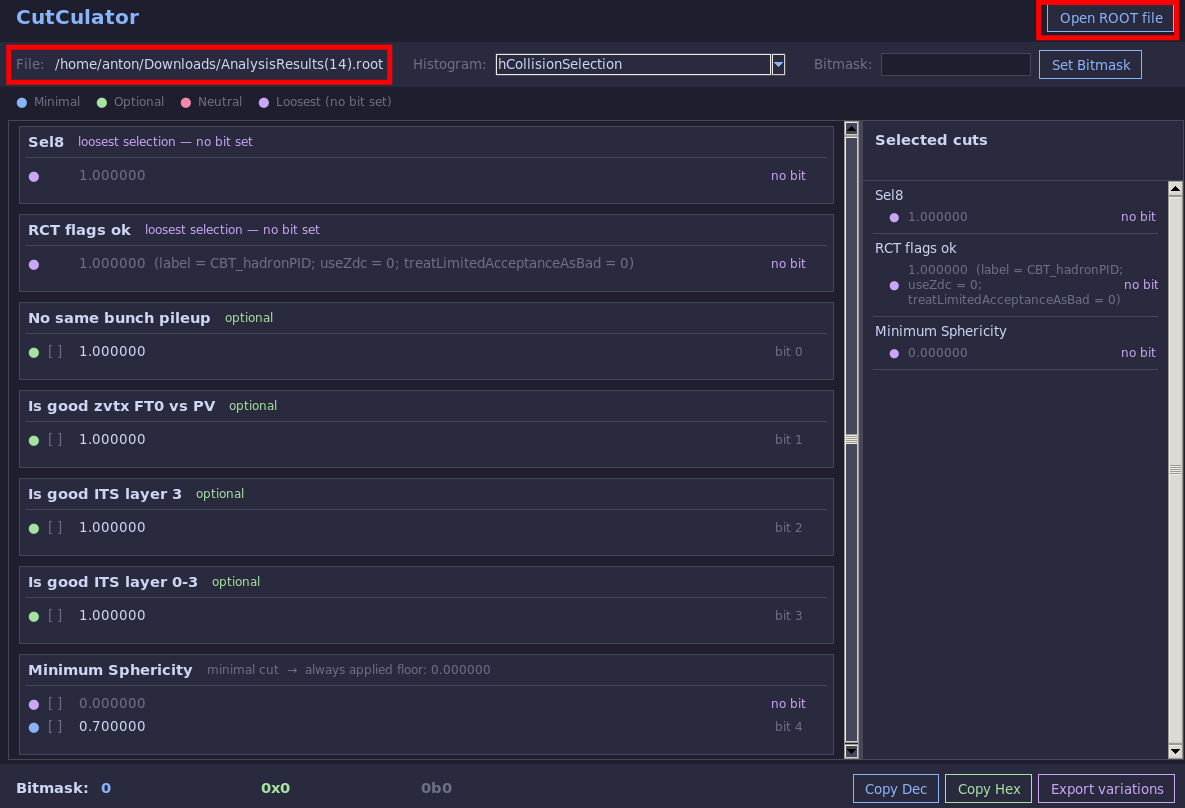
\includegraphics[width=\textwidth,height=0.82\textheight,keepaspectratio]{slides/assets/cutculator-gui-open.png}
        \medskip

        \small Click \textbf{Open ROOT file} to choose a file
        interactively; its path appears next to \textbf{File:}.
        \note{Screenshot supplied by the presenter. The red
                highlights identify the Open ROOT file button at the top
                right and the active file path at the top left. The GUI can
                be launched without a file argument and the producer output
        selected interactively.}
\end{frame}

\begin{frame}[shrink=8]{CutCulator GUI: choose the selection histogram}
        \centering
        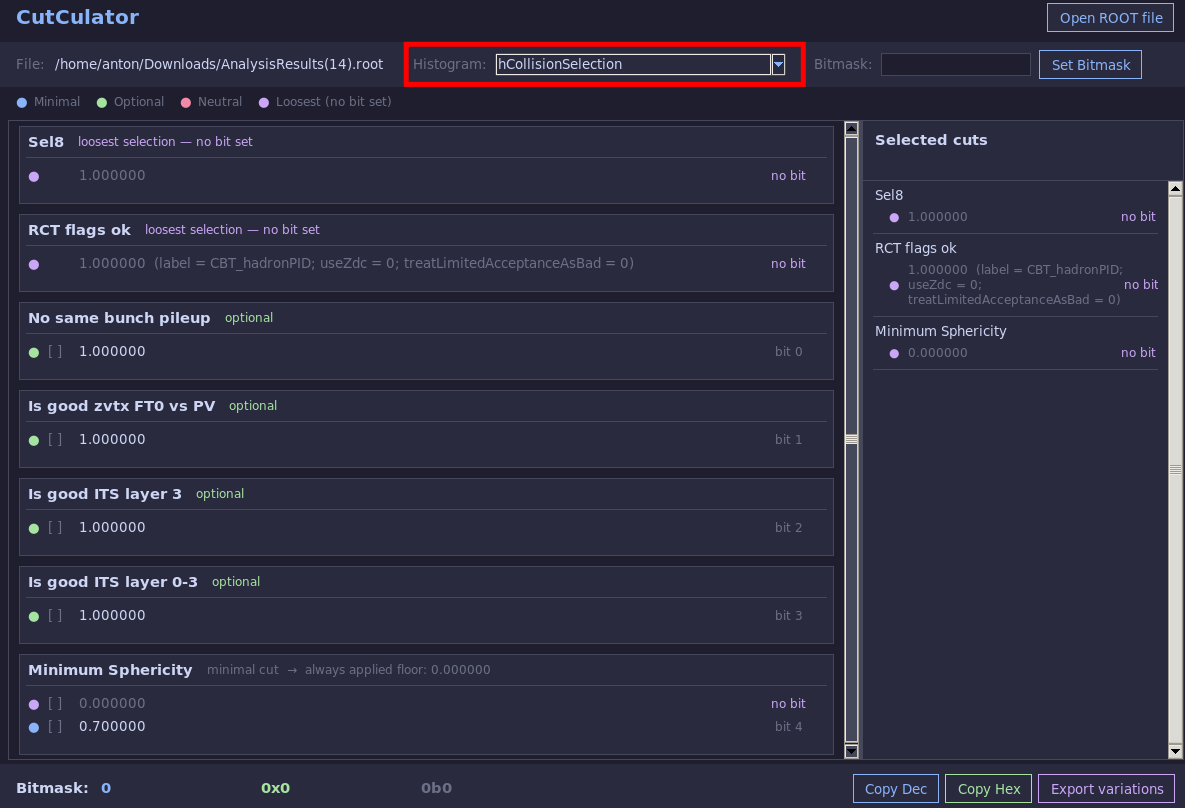
\includegraphics[width=\textwidth,height=0.82\textheight,keepaspectratio]{slides/assets/cutculator-gui-histogram.png}
        \medskip

        \small Use the \textbf{Histogram} dropdown to choose
        collision, track or candidate selections.
        \note{Screenshot supplied by the presenter. The red highlight
                identifies the histogram dropdown, currently showing
                hCollisionSelection. Choose hTrackSelection for tracks,
                hLambdaSelection for Lambda candidates, or the other
        selection histogram corresponding to the desired particle sample.}
\end{frame}

\begin{frame}{CutCulator GUI: select cuts and copy the mask}
        \centering
        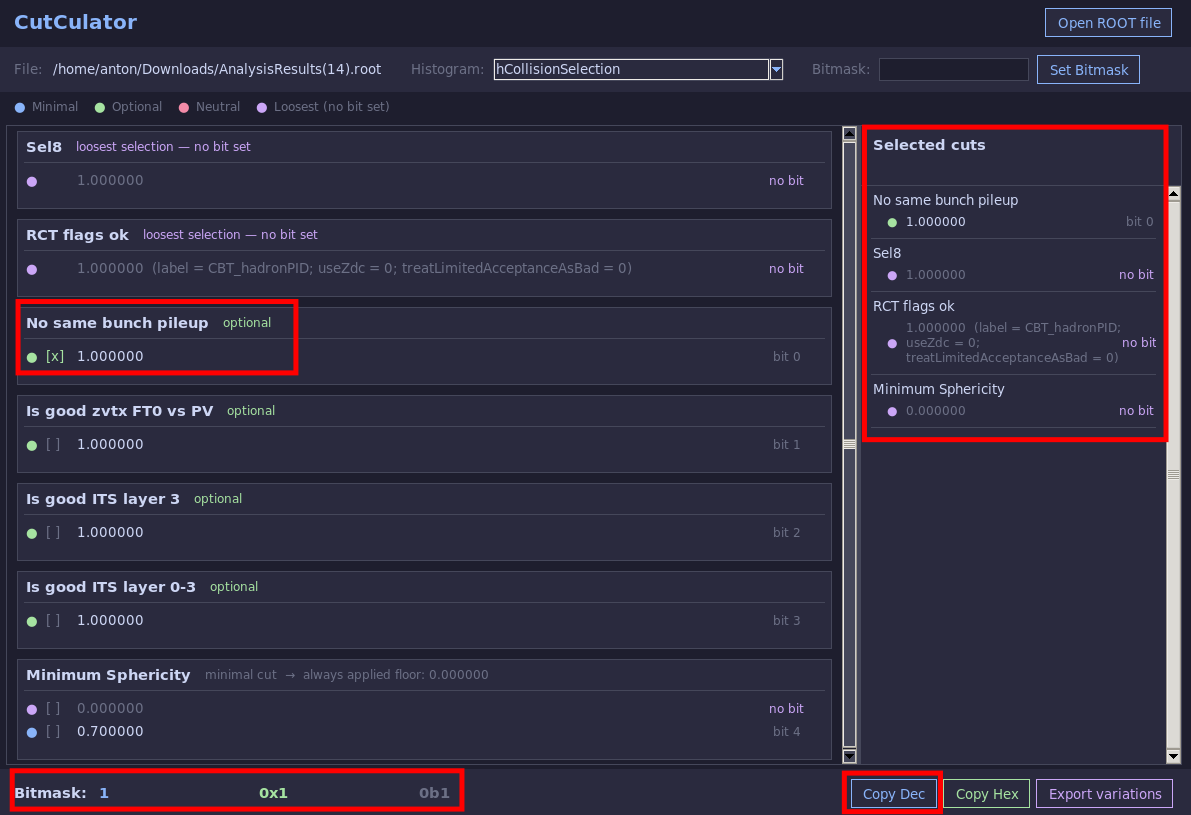
\includegraphics[width=\textwidth,height=0.75\textheight,keepaspectratio]{slides/assets/cutculator-gui-selection.png}
        \medskip

        \small Check a selection on the \textbf{left}; review its
        summary under \textbf{Selected cuts} on the right.\par
        The \textbf{Bitmask} updates at the bottom; use \textbf{Copy
        Dec} or \textbf{Copy Hex} to copy it.
        \note{Screenshot supplied by the presenter. The highlighted
                No same bunch pileup option is selected, setting bit 0. The
                Selected cuts panel lists the chosen decision along with the
                always-applied no-bit floors. The bottom status shows the
                updated mask as decimal 1, hexadecimal 0x1 and binary 0b1.
        Copy Dec copies the decimal form; Copy Hex copies the hexadecimal form.}
\end{frame}

\begin{frame}{CutCulator GUI: inspect a filter histogram}
        \centering
        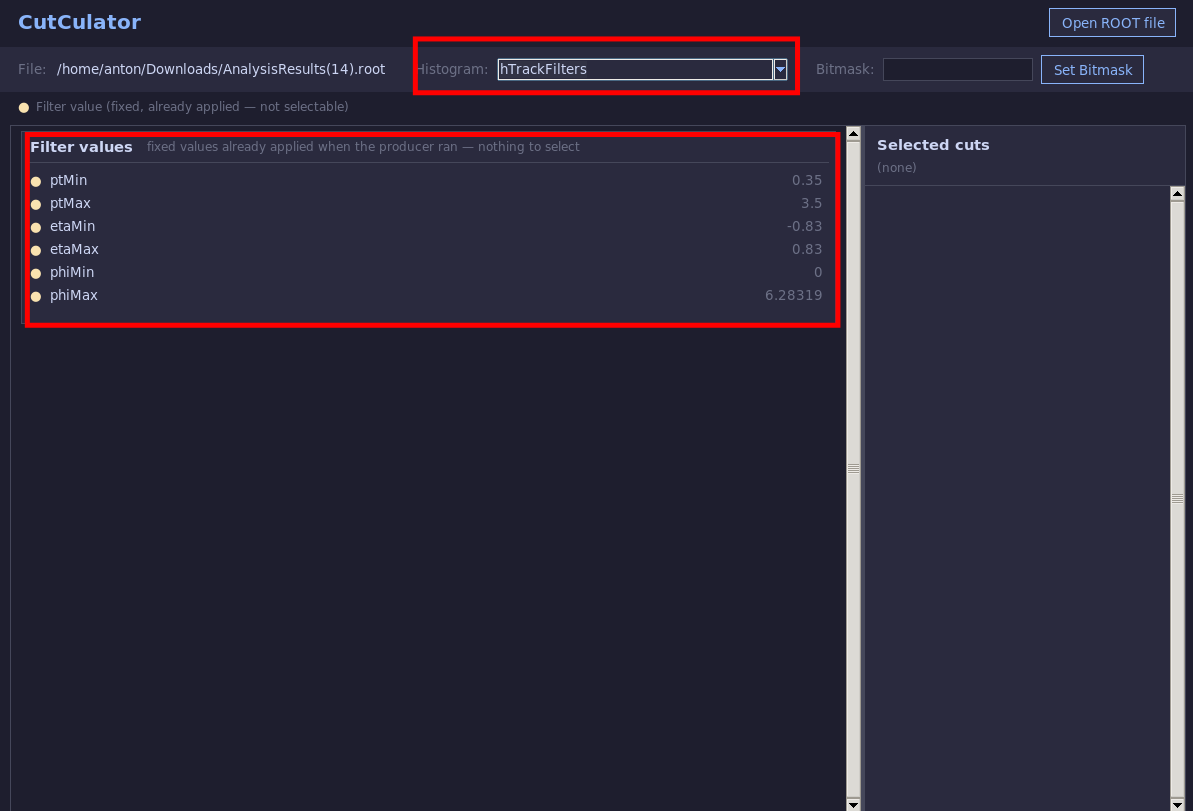
\includegraphics[trim=0 460 0
        0,clip,width=\textwidth,height=0.65\textheight,keepaspectratio]{slides/assets/cutculator-gui-filters.png}
        \medskip

        \raggedright
        Choose \texttt{hTrackFilters} to inspect the producer's track
        prefilters.
        \begin{itemize}
                \item The displayed values were already applied
                        during production.
                \item They are read-only: there are no selection bits
                        to choose here.
        \end{itemize}
        \note{Screenshot supplied by the presenter. The image is
                clipped in LaTeX to omit the empty lower part of the window.
                The highlighted dropdown shows hTrackFilters; the values
                panel records ptMin, ptMax, etaMin, etaMax, phiMin and phiMax
                from this production. Unlike a selection histogram, this view
        offers no checkboxes and no bitmask choices.}
        \src{O2Physics/PWGCF/Femto/Macros/cutculator_gui.py}
\end{frame}

\begin{frame}[fragile,shrink=8]{Optional: a terminal-only CutCulator}
        A terminal-only version is available when needed, for example
        over SSH without a graphical display. It computes the same selection
        masks; the GUI is generally easier to use.
        \medskip\par
 \begin{lstlisting}[language=bash]
 O2PHYSICS_SRC="$HOME/alice/O2Physics"
 python3 "$O2PHYSICS_SRC/PWGCF/Femto/Macros/cutculator.py" \
   AnalysisResults.root
 \end{lstlisting}

 \begin{lstlisting}[language=bash]
 # Inspect the cuts represented by an existing mask:
 python3 "$O2PHYSICS_SRC/PWGCF/Femto/Macros/cutculator.py" \
   AnalysisResults.root --bitmask
 \end{lstlisting}
        \small Decode mode asks for the histogram and then the mask.\par
        \note{TUI here means line-based terminal prompts. Indices are
                generated from the file, so demonstrate rather than hard-code
                an index. A no-bit minimal floor contributes zero to the mask
                but is still in effect. The --bitmask flag is verified in
        this local checkout and may differ in other versions.}
        \src{O2Physics/PWGCF/Femto/Macros/cutculator.py}
\end{frame}

\begin{frame}{CutCulator in the terminal: choosing a histogram}
        \centering
        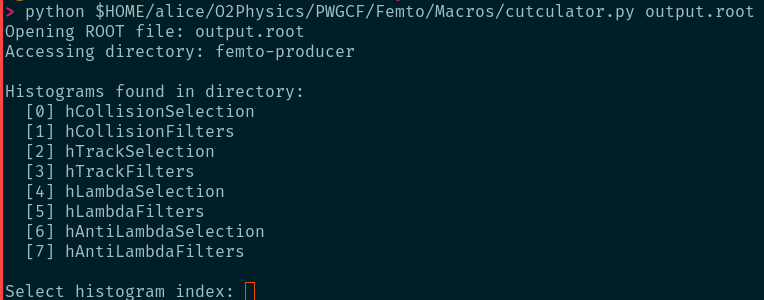
\includegraphics[width=\textwidth,height=0.66\textheight,keepaspectratio]{slides/assets/cutculator-terminal.png}
        \medskip

        \raggedright
        \textbf{Example:} enter \texttt{2} for
        \texttt{hTrackSelection}, or \texttt{4} for
        \texttt{hLambdaSelection}.\par
        \small The indices depend on the histograms in your producer output.
        \note{Screenshot supplied by the presenter. Here the producer
                QA file is called output.root. It contains the same kind of
                selection metadata described for AnalysisResults.root. Choose
                a selection histogram to compute a mask; filter histograms
        only describe fixed prefilters.}
\end{frame}

\begin{frame}{CutCulator in the terminal: selected cuts and final mask}
        \begin{columns}[c]
                \begin{column}{.67\textwidth}
                        \centering
                        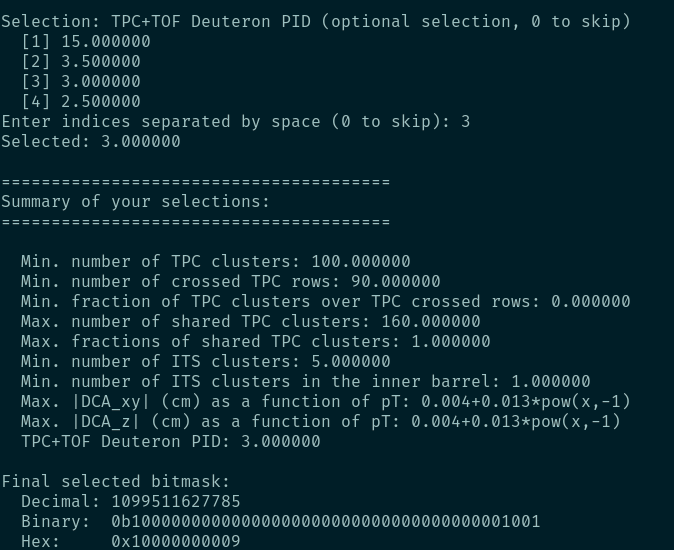
\includegraphics[width=\textwidth,height=0.85\textheight,keepaspectratio]{slides/assets/cutculator-summary.png}
                \end{column}
                \begin{column}{.30\textwidth}
                        \small
                        \textbf{Check the selected cuts}\par
                        The summary lists the thresholds chosen for the sample.
                        \medskip

                        \textbf{Read the final mask}\par
                        Decimal, binary and hexadecimal are three
                        representations of the same integer.
                        \medskip

                        Copy the mask into the corresponding
                        particle-selection configurable.
                \end{column}
        \end{columns}
        \note{Screenshot supplied by the presenter. This example
                selects a TPC+TOF deuteron PID threshold of 3 and prints the
                chosen track-quality and PID selections followed by the final
                mask. The mask is specific to this producer's configuration
                and must not be reused for a different production without
        checking its metadata.}
\end{frame}
